\begin{artengenv}{Piotr Błaszczyk}
	{Galileo's paradox and numerosities}
	{Galileo's paradox and numerosities}
	{Galileo's paradox and numerosities}
	{Pedagogical University of Cracow, Institute of Mathematics}
	{Galileo's paradox of infinity involves comparing the set of natural numbers, $\N$, and the set of squares, $\{n^2:\, n\in\N\}$. Galileo \parencite*{ref_GG38},  by setting up a one-to-one correspondence, considers these sets  to have equal \textit{number} of elements. Then, he characterizes the set of squares as \textit{smaller} than the set of all numbers on the intuitive ground that ``there are many more numbers than squares.''  
	Finally, he concludes that infinities do not comply with the law of trichotomy when compared in terms of greater--lesser.
	
	Cantor's cardinal numbers provide a now-standard measure for sets. Cantor \parencites*{ref_C97}[Engl. transl.][]{ref_C15}  defines the relation greater--lesser and proves the law of trichotomy for these numbers. 
	When they apply to subsets of $\N$,   any set can be either finite or of the power $\aleph_0$. Although  $\N$  includes squares, these two sets are of the same cardinality.
	
	Cantor's ordinal numbers {measure}  well-ordered sets. Then, the same number $\omega$  identifies the order type of the sets  $\mathbb N$ and \mbox{$\{n^2:\, n\in\N\}$}.
	
	Benci and Di Nasso \parencite*{ref_BN19} introduce specific numbers called \textit{numerosities}  to  measure sets. In that theory,  the following claim is true: \textit{numerosity of A} $<$ \textit{numerosity of B}, whenever $A\subsetneq B$. Numerosities, like  ordinal numbers,  require some structure on measured sets called labels.
	
	In this paper, we present a simplified, self-contained version of the theory of \textit{numerosities} that applies to subsets of $\N$ with the \textit{natural} order and does not refer to labels. This theory complies with Galileo's presupposition that when $A\subsetneq B$, then
	the \textit{number} of  elements in $A$ is  smaller than the \textit{number}  of  elements in $B$. Specifically, we show that given the \textit{numerosity} of $\N$ is the specific hyperreal number $\alpha$, the \textit{numerosity} of the set of squares is the integer part of the number $\sqrt{\alpha}$, that is $\big\lfloor\sqrt{\alpha}\big\rfloor$, and  the inequality  $\big\lfloor\sqrt\alpha\big\rfloor<\alpha$ holds.
	
	In the second part, we discuss  Euclid's axiom \textit{The whole is greater than the part},  praised by founders of the numerosity theory,  and  Mancosu's \parencite*{ref_pm09},  the first study that introduced numerosities into a philosophical debate.  To this end, we embed number systems referred to in the paper---hyperreals, numerosities, Cantor ordinal numbers, and algebraic interpretation of Euclid's axiom---in the ordered field of Conway numbers.}
	{non-standard real numbers, numerosities, cardinal numbers, Galileo's paradox.}






%\newpage\tableofcontents
%\newpage
\section{Introduction}
\vspace*{-30pt}
\subsection{1.1. Galileo on infinities}
\lettrine[loversize=0.13,lines=2,lraise=-0.01,nindent=0em,findent=0.2pt]%
{I}{}n  \textit{Discorsi e dimostrazioni matematiche: intorno à due nuoue scienze, attenenti alla mecanica \& i~movimenti locali\ldots{}} \parencite*{ref_GG38}, in a series of dialogues, Galileo Galilei discusses many topics in natural philosophy.  Whether a line consists of  points was then a routine question. 
Euclid's \textit{Elements} and Aristotles' \textit{Physics} set up that issue.  
Definition VII.2 of the \textit{Elements}, ``A number (is) a multitude 
(\foreignlanguage{polutonikogreek}{pl~hjos}) composed of units (\foreignlanguage{polutonikogreek}{mon'awn})'', ascertain numbers consist of units.  
The question was whether in geometry, the realm of continuity, points, defined by  I.1 ``A point is that of which there is no part'', could play a role analogous to units in arithmetic.
 Aristotles'  definition that  continuous objects are ``divisible into  infinitely (\foreignlanguage{polutonikogreek}{>ae'i}) divisible divisibles'' (\textit{Physics} VI.2) introduce infinity into the debate.


Galileo's position that magnitudes are composed of  \textit{non quanti} indivisibles drives him to the then-known paradox of infinity of parts of line segments. Yet, he
gives that discussion  a new push
by turning it into whether infinities, alike magnitudes, and numbers, are comparable in terms of greater-lesser.
His initial argument is simple:
Since one line can be greater than another, given each contains ``an infinite number of points'',  the infinity of points in the longer one is greater than the infinity of points in the shorter \parencite[see][30--33]{ref_GG56}. 

At this stage, greater-lesser does not mean set-subset relation. The idea of comparing line segments, rather than their lengths (measures), originates from the \textit{Elements}. It was self-evident in the 17\textsuperscript{th} century and prevailed until the 19\textsuperscript{th} century. The rise of the real number system enhanced the process of measuring 
magnitudes---lines by lengths, figures by areas, solids by volumes.  
Both in ancient Greek and 17\textsuperscript{th}-century mathematics, it was also evident,  that line segments were subject to the law of trichotomy (see section \S\,5.1 below). Thus, the point was whether infinities are subject to the same laws as then-common mathematical objects, such as line segments,  natural numbers, or ratios.

The idea that there is a variety of infinities,  one greater than another, puzzled the discussants.  Galileo  does not  reject the infinity, instead  he concludes that the law of  trichotomy does not apply in that domain:
``we cannot speak of infinite quantities as being the one greater or less than or equal to another'' \parencite[30]{ref_GG56}. 
To clarify this point, he involves natural numbers and states what later got the name Galileo's paradox of infinity.   
He sets up a one-to-one correspondence between the set of natural numbers, $\N$, and the set of squares, $\{n^2: n\in\N\}$; in this sense, respective infinities  are equal.
 He also observes that ``there are more numbers than squares;'' in this sense, the former infinity is greater than the latter.  Here is the key part of this dialogue \parencite[33]{ref_GG56}:
 
\myquote{
If I should ask further how many squares there are one might reply truly that there are as many as the corresponding {number} of roots, since every square has its own root and every root its own square, while no square has more than one root and no root more than one square [...]. 
But if I inquire how many roots there are, it cannot be denied that there are as many as the numbers because every number is the root of some square. This being granted, we must say that there are as many squares as there are numbers because they are just as {numerous} as their roots, and all the numbers are roots
[...]  Yet at the outset we said that there are many more numbers than squares, since the larger portion of them are not squares. 
}

The conclusion is as follows: 
\myquote{
we can only infer that the totality of all numbers is infinite, that the number of squares is infinite, and that the number of their roots is infinite; neither is the number of squares less than the totality of all the numbers, nor the latter greater than the former; and finally the attributes \textit{equal}, \textit{greater}, and \textit{less}, are not applicable to infinite, but only to finite, quantities. When therefore Simplicio introduces several lines of different lengths and asks me how it is possible that the longer ones do not contain more points than the shorter, I answer him that one line does not contain more or less or just as many points as another, but that each line contains an infinite number \parencite[33]{ref_GG56}.
}


%Hence, on the one hand, the infinity of all numbers and  the infinity of all squares, are equal, in the sense one-to-one correspondence, on the other hand, the set of all numbers  is greater than the set of square, since it includes the later.  

In the dialogue that  follows, Galileo also argues that one can not compare finite and infinite in terms of 
greater--lesser, as that gives rise to new paradoxes; 
``And thus from your ingenious argument we are led to 
conclude that the attributes \textit{larger}, \textit{smaller}, and \textit{equal}
have no place either in comparing infinite quantities with each 
other or in comparing infinite with finite quantities'' \parencite[33]{ref_GG56}. 

\subsection{1.2. Cantor's  law of trichotomy for cardinal numbers}
Georg Cantor, in  philosophical 
digressions spread throughout his mathematical papers presents himself as the pioneer of a study of actual infinity. In his view,   only  Leibniz and Bolzano had approached the absolute infinity seriously before he did. His biographer, Joseph Dauben, in the very popular book \textit{Georg Cantor. His Mathematics and Philosophy of the Infinite} \parencite*{ref_jd}, upholds this legend. At present,  Cantor is generally considered the founding father of the mathematical study of infinity.  However,  there were pre-Cantorian theories of actual infinity developed within the tradition of geometrical optics, from Euclid, through Kepler to Descartes \parencite[see][]{ref_pb20}. And the real challenge for Cantor was  Euler's \textit{Introductio in Analysin Infinitorum} \parencite*{ref_LE48} which refers to the study of infinity in its very title and, obviously, the substance content. Since Euler's infinite numbers were inverses of infinitesimals, Cantor made endless attempts to dismiss these seemingly strange numbers \parencite[see][]{ref_bf}. Nevertheless, he neither mentioned Euler as the author of a competing theory of infinity, nor Galileo and his idea of equality of infinities based on one-to-one correspondence. 

Nowadays, Cantor's theory of cardinal numbers is a part of the common mathematical and philosophical education. Therefore, here, by referring to \parencite{ref_C97}, we note only the basic definitions related to Galileo's paradox.   Thus, the cardinal number of a set $M$, $\overline{{\overline M}}$, is equal to  the cardinal number of  a set $N$,
 $\overline{{\overline N}}$,  iff there is a one-to-one correspondence between these sets, $M\sim N$.   The relation greater--lesser does not reduce to the relationship of one set being a subset of another.  It is defined as follows:  $\overline{{\overline N}}< \overline{{\overline M}}$ iff there is $L\subset M$ such that $L\sim N$ and it is not the case that $N\sim M$.   Cantor managed to prove the law of trichotomy for cardinal numbers. Yet, it was far from trivial, as he observed:
\myquote{
We have seen that, of the three relations  $\textbf{a}=\textbf{b},\ \textbf{a}<\textbf{b},\ \textbf{a}>\textbf{b}$
each one excludes the two others. On the other 
hand, the theorem that, with any two cardinal 
numbers $\textbf{a}$ and $\textbf{b}$, one of those three relations must 
necessarily be realized, is by no means self-evident 
and can hardly be proved at this stage \parencites{ref_C97}[English translation after][90]{ref_C15}.\footnote{In the current set theory,  the law of trichotomy for cardinal numbers is equivalent to the Axiom of Choice. See \parencite[ch. 8, \S\,6.]{ref_km78}.}
}

At the turn of the 19\textsuperscript{th} and 20\textsuperscript{th} centuries, Cantor's theory of infinity reigned.  Although its definitions are not built on  theorems, as it sometimes happens in mathematics, people started to consider cardinal numbers as the indispensable measure of infinite sets.

Kurt G\"odel reinforced the belief that there is no alternative to Cantor's theory of infinite
numbers. 
In \parencite{ref_kg47}, he presents
cardinal numbers as extending the system of natural numbers $(\N,+, \cdot, 0, 1,<)$ and seeks
to show that ,,this extension can be effected in a uniquely determined manner.''

Nevertheless, there is still some  dissatisfaction: when we apply Cantor's theory to subsets of $\N$ there are only two possibilities there---a set can be either finite
or has the cardinality $\aleph_0$. 

Ordinal numbers provide another way of measuring infinite sets, yet they refer to well-ordered sets rather than bare sets. Cantor designed arithmetic for these numbers as well as the greater-lesser relation. In this case, the law of trichotomy does not relate to the Axiom of Choice  \parencite[see][ch. 7]{ref_km78}. Modern accounts of set theory introduce cardinal numbers as specific ordinal numbers \parencite[ch. 3]{ref_tj}.
Finite numbers, that is, elements of $\mathbb N$, are both cardinal and ordinal numbers, and in each case, they contribute the hierarchy greater-lesser.




\subsection{1.3. Numerosities}
In  the sections that follow, we present a theory that assigns  special numbers, called \textit{numerosities}, to subsets of $\N$ in  such a way that \textit{numerosity of A}$<$\textit{numerosity of B}, whenever $A\subsetneq B$. In this sense, \textit{numerosities} meet Gelileo's intuition that the relation greater--lesser between infinities agrees with the subset relation. 

The general theory of \textit{numerosities} is developed in \parencite{ref_BN19} as well as a variety of papers also authored by Vieri Benci and his collaborators. Below, we present its simplified version that applies only to subsets of $\N$. We define \textit{numerosities} as nonstandard natural numbers introduced through an ultrapower construction, where the \textit{numerosity} of $\N$ is a number $\alpha$ represented by the equivalence class $[(1,2,3,...)]$. 
Still, we need a bigger structure  to define numbers such as $\sqrt \alpha$ or $\alpha/2$. To this end, we introduce a field of nonstandard real numbers.

  To make this presentation self-contained, we start with the basics of the theory of ordered fields. Then, we proceed to the extension of the field of real numbers to the field of nonstandard reals. With these foundations, we can easily introduce \textit{numerosities} and demonstrate  theorems. 




\section{The basics of ordered fields theory}


A commutative field $(\F,+,\cdot,0,1)$ together with a total order $<$ is an ordered field when the sums and products are compatible with the order, that is
%\begin{eqnarray*}
%x<y &\Rightarrow& x+z<y+z,\\
%x<y,\, 0<z&\Rightarrow& xz<yz.
%\end{eqnarray*}
\[x<y \Rightarrow x+z<y+z,\ \ \ x<y,\, 0<z\Rightarrow x\cdot z<y\cdot z.\]

In any ordered field, we  define in a usual way an absolute value, $|x|$,  and a limit of  sequence,  
\[\lim\limits_{n\rightarrow\infty}a_n=g  \Leftrightarrow (\forall \varepsilon >0)(\exists k\in\N)(\forall n\in\N)(n>k \Rightarrow |a_n-g|<\varepsilon).\]


Note, however,  that while in real analysis the formula $\forall \varepsilon>0$
stands for $\forall \varepsilon\in\R_+$, in an ordered field,  it means
$\forall \varepsilon\in\F_+$. Moreover, in any field, whether Archimedean or non-Archimedean, indexes $k, n$ range over standard natural numbers $\N$. 

 The term $n$ is defined by
\[n=_{df}\underbrace{1 +1 + ... + 1}_{n - times},\]
while $\frac nm=_{df} n\cdot m^{-1}$. On this, basis we assume that any ordered field includes natural numbers, $\N$, and rational numbers, $\Q$. In fact, the field of fractions $(\Q,+,\cdot,0,1,<)$ is the \textit{smallest} ordered field.

In every ordered field, we can define the following subsets of $\F$:
\begin{eqnarray*}
 \mathbb L &= & \{x\in \F: (\exists n\in \N)(|x|<n)\},\\
 \mathbb A &=&   \{x\in \F: (\exists n\in \N)(\tfrac 1 n<|x|<n)\},\\
 \Psi             &=& \{x\in \F: (\forall n\in \N)(|x|>n)\},\\
 \Omega      &=& \{x\in \F: (\forall n\in \N)(|x|<\tfrac 1n)\}.
 \end{eqnarray*}

 The elements of these sets are called  limited, assignable,   infinite, and infinitely small numbers respectively.
Here are some obvious relationships between these kinds  of elements, we will call them $\Omega\Psi$ rules,
%In what follows we show some relations and dependencies we will refere to when interpreting Euler's writings.
%We can easily show  infinite numbers can be equally definied via  natural numbers, finite numbers, as well as assignable numbers
%It can be easily shown that the following relations hold (in short, $\Omega\Psi$ rules):
\begin{enumerate}\itemsep 0mm
\item[] $(\forall x, y\in\Omega)( x+y\in\Omega, x\cdot y\in\Omega)$,
\item[]  $(\forall x\in\Omega)( \forall y\in\mathbb L)( x\cdot y\in\Omega)$,
\item[] $(\forall x)(x\in \mathbb A\Rightarrow  x^{-1}\in\mathbb A)$,
\item[] $(\forall x\neq 0)(x\in\Omega  \Leftrightarrow \ x^{-1}\in\Psi)$.
\end{enumerate}


%\begin{equation} \Psi= \{x: (\forall a\in\A)(|x|>|a|)\}. \end{equation}
%\begin{equation} \Omega=\{x: (\forall a\in\A)(|x|<|a|)\}. \end{equation}
%\begin{equation}(\forall x, y\in\Omega)( x+y\in\Omega, xy\in\Omega) \end{equation}
%\begin{equation}(\forall x\in\Omega)( \forall y\in\mathbb A)( xy\in\Omega)\end{equation}
%\begin{equation}(\forall x)(x\in \mathbb A\Rightarrow  x^{-1}\in\mathbb A)\end{equation}
%\begin{equation}(\forall x\neq 0)(x\in\Omega  \Leftrightarrow \ x^{-1}\in\Psi),\end{equation}
%\begin{eqnarray*}(\forall x, y\in\Omega)&& x+y, xy\in\Omega,\\
%(\forall x\in\Omega)( \forall y\in\mathbb L)&&  xy\in\Omega,\\
%(\forall x\in \Omega)(\exists y\in\Psi)&& xy\in \mathbb L,\\
%(\forall x\neq 0) && x\in\Omega  \Leftrightarrow \ x^{-1}\in\Psi,\\
%(\forall x\in \mathbb A) &&  x^{-1}\in\mathbb A.
%\Omega=\{x: (\forall a\in \mathbb A)(|x|<|a|)\}
%\end{eqnarray*}

%Referring to the set $\Omega$, an equivalence relation is defined by
%\[x\approx y \Leftrightarrow x-y \in\Omega.\]
%We say that $x$ \emph{is infinitely close to} $y$, when the relation $x\approx y$ holds.


%Although we present the above relations within the modern framework, all of them were explicitly discussed in \parencite{Euler:55}, ch. 3.
%Next to $\Omega\Psi$ rules, it can also  be shown that $\Omega$ is the maximal ideal in the ring $(\mathbb L,+,\cdot,0,1)$ and the quotient ring $\mathbb L/{\Omega}$ is a field.  We do emphasize   $\Omega\Psi$  rules only because they are explicitly discussed in (Euler 1755);  see  \S \ below.


\subsection{2.1. Archimedean axiom}
When to the axioms of an ordered field we add the so-called Archimedean axiom, we obtain the class of
Archimedean fields.
Here are some equivalent forms of the Archimedean axiom:
\begin{enumerate}\itemsep 0mm
  \item [(A1)] $(\forall x,y\in \F)(\exists n\in\N)(0<x<y\Rightarrow n\cdot x>y)$,
  \item [(A2)] $(\forall x\in\mathbb F)(\exists n\in\N)(n>x) $,
  \item [(A3)] $\lim\limits_{n\to \infty} \frac 1n=0$,
  \item [(A4)] $(\forall x,y\in\mathbb F)(\exists q\in\mathbb Q)( x<y\Rightarrow x<q<y),$
\item [(A5)] For any Dedekind cut  $(A,B)$ of $(\F,<)$ obtains\footnote{For the remainder, a pair $(A,B)$
 of non-empty sets is a Dedekind cut of a totally ordered set $(X,<)$ iff: (1) $A\cup B=X$, %(2) $A\neq \emptyset, B\neq\emptyset$, (3)
 (2) $(\forall x\in A)(\forall y\in B)(x<y)$.}
$$(\forall n\in\mathbb{N})(\exists a\in A)(\exists b\in B)(b-a<\tfrac 1n),$$
\item[(A6)] $\Omega=\{0\}$.
\end{enumerate}



Versions A1 and A2 are well-known,  both in the mathematical as well as the historical context. A1 in the following form $(\forall x,y\in \F)(\exists n\in\N)(nx>y)$ originates from Euclid's \textit{Elements}, Book V, definition 4. It characterized the ancient Greek structure of magnitudes, specifically, line segments. In modern times, it is an axiom of Euclidean geometry.  Calculus courses usually present A3 as a theorem. However, it  follows from some versions of the continuity of real numbers, for example, C1 or C2 as presented below, 
or is explicitly included in other versions.
  A6 reveals that in a non-Archimedean field, the set of infinitesimals contains at least one positive element, say $\varepsilon$.
     Then, by $\Omega\Psi$ rules, $\tfrac \varepsilon n$, as well as, $n\cdot\varepsilon$   are also infinitesimals.

A3 provides a neat characterization of the non-Archimedean field: $(\frac 1n)$ is not a null-sequence.
In the field of formal power series (Laurent series), given $0<x<1$, $(x^n)$ is a null-sequence, that is \mbox{$\lim\limits_{n\to \infty}x^n=0$}. Moreover, it is a non-Archimedean and Cauchy-complete field \parencites[see][70]{ref_ce}[or][269--272]{ref_pb07}. The field of hyperreals, as defined in the next section, is also non-Archimedean and Cauchy-complete. Yet, due to the so-called saturation principle, there are no null sequences, except constant ones (or constant but a finite set).  

 
     
     
      %In addition,    inverses of these elements, i.e.  $\tfrac n \varepsilon$, $\tfrac 1 {n\varepsilon}$, also belong to that field and according to $\Omega\Psi$ rules, these are  infinitely large numbers. Let $\Omega_0$ stand for the set of non-zero infinitesimals, i.e.   $\Omega_0=\Omega\setminus\{0\}$.

%The  versions A1 to A6 above are equivalent within the framework of an ordered field while  some of them, for instance A1, apply to an ordered group
%$(\mathbb G, +,<)$. Then, the term $nx$ is defined by
%\[nx=_{df}\underbrace{x +x + ... + x}_{n - times}.\]
%
% We can also apply versions A4 and A5, provided the concept of fraction is interpretable in a group. Versions A3 and A6 involve the concept of an absolute value. While the very definition makes sense in any ordered group, some properties of the absolute value, such as
%$|x\cdot y|=|x|\cdot|y|$,
% require the order to be compatible both with sums and products. Hence, these versions need to be applied carefully.
%
% At the end of the 19\textsuperscript{th} century, a few non-Archimedean structures were introduced, however they contained rather exotic mathematical entities that provoked distrust.\footnote{\parencite{Ehrlich:06} provides a thorough overview of these structures.}
%We present a non-Archimedean group  made up  of then well-known objects, namely complex numbers; the simplicity of the model makes us wonder why it was not involved in the dispute concerning infinitesimals.
%
%Let $(\mathbb C,+,0,\prec)$ be the additive group of complex numbers with the lexicographical order, i.e.,
%\[a+bi\prec  c+di \Leftrightarrow a<c \vee  (a=c,\,b<d).\]
%
% The order is compatible with sums,  although  not  with products. One can easily show that
% $0\prec i\prec 1$,
%  moreover,   for every natural number $n$ the inequality $ni\prec 1$ holds. The set $\{ri:r\in \R\}$ includes  infinitesimals of the group $(\mathbb C,+,0,\prec)$.\footnote{\parencite{Blaszczyk:13b} provides historical account of the Archimedean axiom, from Euclid and Archimedes, through Heiberg's edition of Greek text, to the 19\textsuperscript{th} century theories of magnitudes developed by Stolz, Weber, H\"older and others. }
%\end{document}

\subsection{2.2. Real numbers}

 The field of real numbers   is  defined as a commutative ordered field $(\mathbb F,+,\cdotp,0,1,<)$ in which
 every Dedekind cut $(L,U)$ of $(\F,<)$ satisfies the following condition:
\begin{equation}\tag{C1}(\exists x\in\F)(\forall y\in L)(\forall z\in U)(y\leq x\leq z).
\end{equation}


Here are some  equivalent forms of C1:

\begin{enumerate}\itemsep 0mm
\item [(C2)] If $A \subset \F$ is a nonempty set which is bounded above, then there exists $a \in \F$ such  that  $a = \sup A$.
\item [(C3)] The field  is Archimedean and every Cauchy (fundamental) sequence $(a_n)\subset \F$  has a limit in $\F$.
\item[(C4)] The field  is Archimedean  and
 if $\big\{A_{n}|\ n\in\mathbb{N}\ \!\big\}\subset \F$ is a family of descending, closed line segments, then $\bigcap\limits_{n\in\mathbb{N}} A_{n}\not=\emptyset.$
\end{enumerate}


%Any equivalent form of C1  usually gets the name of {continuity} or {completeness},  and then the real numbers system is called the {continuous ordered field} or the {complete ordered field}. The version C2 is also known as {Dedekind completeness} or the {least upper bound} (LUB) principle, whereas   the second part of C3 is called  Cauchy completeness.  Since Dedekind and Cauchy completeness are not equivalent,  we prefer to use more specific names like Dedekind cut  or LUB principle.

The above definition applies the theorem that every two ordered fields satisfying C1 are isomorphic. In this sense, the field of real numbers is the unique, complete ordered field. Moreover, any Archimedean field is isomorphic to a subfield of real numbers.  As a result, any field extension of real numbers is non-Archimedean and includes infinitely small and infinite numbers.  
\section{The field of hyperreals}

In this section, we provide a specific field-extension of real numbers, namely a field of hyperreals (non-standard real numbers). Since \parencite{ref_RA}, many different approaches to non-standard reals have been developed. The one presented below is based on the so-called ultrapower construction.  The set of hyperreals  $\R^*$  is defined as the quotient class of the set of sequences of real numbers, $\R^{\N}$, with  respect to a specific relation defined on the set of indexes $\N$. We begin with this relation.


\subsection{3.1. Ultrafilter on the set $\N$}

 We start with
 the definition of an ultrafilter  on  $\N$ and present some basic results concerning ultrafilters.

  \textbf{Definition 1} A family of sets $\mathcal U\subset \mathcal P (\N)$ is an
  ultrafilter on $\N$ if (1) $\emptyset \notin \mathcal U$, (2) if $A,B\in\mathcal U$,
   then $A\cap B\in\mathcal U$, (3) if $A\in\mathcal U$ and $A\subset B$,
   then $B\in\mathcal U$, (4) for each  $A\subset \N$, either $A$ or its
   complement $\N\setminus A$ belongs to $\mathcal U$.

%It follows from this definition that either the set of odd numbers or the set of even numbers belongs to an ultrafilter.

   Take the family of  sets with  finite complements,
   \[\{A\subset\N:  \N\setminus A\ \ \mbox{is\ finite}\}.\]

It  is usually called the Fr\'{e}chet  filter on $\N$. Indeed, it obviously  satisfies conditions (1)--(3) listed in  Definition 1. Note, however, that neither the set of odd numbers nor the set of even numbers has a finite complement, hence, the Fr\'{e}chet  filter is not an ultrafilter.
   Still, by  applying the Axiom of Choice it can be  extended to an
ultrafilter. In what follows, let $\mathcal U$ be a fix ultrafilter on $\N$ which extends the
 Fr\'{e}chet  filter.\footnote{Since we apply the fixed ultrafilter, we can refer to the field, rather than a field of hyperreals.    Assuming the continuum hypotheses, $\R^*$  is unique up to isomorphism, that is,  it does not depend on a choice of an ultrafilter extending the Frechet filter.}


 Thus, we know that for every $k\in\N$, the family $\mathcal U$ includes the set
\[\N\setminus \{0,1,2,...,k\},\]
since  sets of this kind belong to the Fr\'{e}chet  filter.  Moreover, the set $\N$ also belongs to $\mathcal U$, since it belongs to the  Fr\'{e}chet  filter.
Next,  due to the condition (4) of Definition 1, for any subset $A$ of $\N$, either $A$, or $\N\setminus A$
belongs $ \mathcal U$. We apply this fact to prove, e.g. an equivalence  (1), as explained below.
Finally, it can be shown that the following proposition holds.

\textbf{Theorem 1} For any subsets $A_1,...,A_n$ of $\N$ such that $A_i\cap A_j=\emptyset$, $i\neq j$. If
$\bigcup_{i=1}^{n} A_i\in\mathcal U$, then  $A_i\in \mathcal U$ for exactly one $i$ such that $1\leq i\leq n$.

By applying this proposition, one can show that relations $<^*$ defined on the set $\R^*$ and $\N^*$ are actually total orders.

\subsection{3.2. Extending the field of real numbers}

In this section, we sketch  how to extend the field of real numbers
$(\R,+,\cdot,0,1,<)$  to a non-Archimedean field of
the hyperreals.\footnote{For details, consult \parencites{ref_BM}{ref_pb16}.} The set $\R^*$  is defined as the quotient class of $\R^{\N}$ with
 respect to the following relation
\[(r_n)\mathcal \equiv (s_n) \Leftrightarrow \{n\in\N: r_n=s_n\}\in \mathcal U.\]

Thus, $\R^*=\R^{\N}/_{\mathcal U}$. Clearly, the equality of hyperreals is defined by
\begin{equation}[(r_n)]= [(s_n)] \Leftrightarrow \{n\in\N: r_n=s_n\}\in \mathcal U. \end{equation}

It means that when sequences  $(r_n), (s_n)$ agree on a set of indexes that belongs to $\mathcal U$, 
they determine the same hyperreal number.  For example, suppose that the set of even numbers belongs to the ultrafilter, 
$\{2n: n\in \N\}\in\mathcal U$. If $r_{2n}=s_{2n}$, for every $n$, then $[(r_n)]=[(s_n])$. Therefore, specifically, the following equality holds
\[[(r_n)]=[(0,2,0,4,0,6,...)]=[(1,2,3,4,5,6,...)]=[(s_n)],\]
where the sequence $(s_n)$ is defined by $s_n=n$, and the sequence $r_n$ is defined by $r_n=n$, for even $n$, and
$r_n=0$, for odd $n$.


New sums and products are defined pointwise, that is
\[[(r_n)]+^*[(s_n)]=[(r_n+s_n)],\ \    [(r_n)]\cdot^*[(s_n)]=[(r_n\cdot s_n)].\]

New total order is defined by
\[[(r_n)]<^*[(s_n)]\Leftrightarrow \{n\in\N: r_n<s_n\}\in\mathcal U.\]

Hence, the product and sum of hyperreals $[(r_1,r_2,...)]$ and $[(s_1,s_2,...)]$ gives
$[(r_1\cdot s_1,r_2\cdot s_2,...)]$, and  $[(r_1+ s_1,r_2+ s_2,...)]$ respectively.
The relation
$[(r_1,r_2,...)]<^*[(s_1,s_2,...)]$ holds when, for example, the set $\{n\in\N: r_n<s_n\}$ equals $\N$ minus some finite set (though the definition of order $<^*$  includes also  other cases).


Standard real number, $r\in\R$, is represented by the class $[(r,r,r,...)]$, i.e., the class of a constant sequence $(r,r,r,...)$. Note that the sequence representing standard real number, e.g. 1, can take the same value from some index on, for example
\[1=[(1,1,1,1...)]=[(0,0,1,1,...)].\]

Owing to the above definitions,  we employ the same symbols for real numbers in the standard and non-standard context; we will also employ the same symbols for sums, products and order relation in the standard and non-standard context.

It follows from the notion of ultrafilter that the following relation holds
\begin{equation}[(r_n)]\neq [(s_n)]\Leftrightarrow \{n\in \N:\ r_n\neq s_n\}\in\mathcal U.\end{equation}

Due to this fact, we can control, e.g. an inequality such as this one $[(r_n)]\neq 0$. This fact, in turn, enables to show that the quotient structure is really an ordered field.



In the next section, we  consider hyperreal numbers represented by sequences of natural numbers, that is $[(n_j)]$, where $(n_j)\subset \N$, for instance
\begin{equation}\alpha=[(1,2,3,...)]=[(n)].\end{equation}

According to the definition of product, we have
\[\alpha^2=[(1,2,3,...)]\cdot[(1,2,3,...)]= [(1^2,2^2,3^2,...)]=[(n^2)].\]

Then, the hyperreal number $\frac \alpha 2$ is determined by the following equalities
\[\frac \alpha 2=[(1,2,3,...)]\cdot [(\tfrac 12,\tfrac 12,\tfrac 12,...)] =\big[\big(\tfrac 12,\tfrac 22,\tfrac 32,...\big)\big]=\big[\big(\tfrac n2\big)\big].\]

Similarly, that  is point-wise,  we define the hyperreal number $\sqrt{\alpha}$, namely
\[\sqrt\alpha =\big[\big(\sqrt 1,\sqrt 2,\sqrt 3,...\big)\big]=\big[\big(\sqrt n\big)\big].\]

In a similar way, the floor function  is defined, namely
\[\big\lfloor [(r_j)]  \big\rfloor=[(\lfloor r_j  \rfloor)].\]

Hence, hyperreal numbers  such as
\[\Big\lfloor \frac\alpha 2 \Big\rfloor\ \ \mbox{and}\ \ \big\lfloor \sqrt\alpha\big\rfloor,\]

are represented by sequences of natural numbers, namely
\[\Big\lfloor \frac\alpha 2 \Big\rfloor= \big[\big(\big\lfloor \tfrac n2\big\rfloor\big)\big],\ \ \ \big\lfloor \sqrt\alpha\big\rfloor=  \big[\big(\big\lfloor\sqrt n\big\rfloor\big)\big].   \]

More specifically,
  \[\Big\lfloor \frac\alpha 2 \Big\rfloor= \Big\lfloor\big[\big(\tfrac 12,\tfrac 22,\tfrac 32,...\big)\big]\Big\rfloor= \big[\big(\big\lfloor \tfrac n2\big\rfloor\big)\big]     =[(0,1,1,2,2,3,3,...)],        \]
\[  \big\lfloor \sqrt\alpha\big\rfloor=  \big[\big(\big\lfloor\sqrt n\big\rfloor\big)\big]=
[(\sqrt 1,1,1,\sqrt 4,2,..., 2,\sqrt 9,3,...,3,\sqrt{16},4,...)].   \]

Note that with natural numbers, the following equalities obtain $\lfloor \frac n2 \rfloor + \lfloor \frac n2 \rfloor=n$ or
$\lfloor \frac n2 \rfloor + \lfloor \frac n2 \rfloor +1=n$,
 depending on whether $n$ is even or odd. Similarly, $\Big\lfloor \frac\alpha 2 \Big\rfloor +\Big\lfloor \frac\alpha 2 \Big\rfloor=\alpha$ or $\Big\lfloor \frac\alpha 2 \Big\rfloor +\Big\lfloor \frac\alpha 2 \Big\rfloor+1=\alpha$, depending on whether the set of even numbers belongs or not  to the ultrafilter $\mathcal U$. More specifically,
suppose the set of even numbers belongs to $\mathcal U$. It means that for any sequence $(r_n)$, only elements with 
even indexes, $r_{2k}$, determine the number $[(r_n)]$, as explained above. Now,
 
 \[\Big\lfloor \frac\alpha 2 \Big\rfloor +\Big\lfloor \frac\alpha 2 \Big\rfloor=[(0,\textbf{2},2,\textbf{4},4,\textbf{6},6,... )]=[(1,\textbf{2},3,\textbf{4},5,\textbf{6},...)]=\alpha.\]
 
  
% The final equality obtains because sequences $(0,2,2,4,4,...)$ and $(1,2,3,4,...)$ agree on the set of indexes
% $\{2n:\ n\in\N\}$.
 
% Yet,  we skip
% a  discussion  needed to justify this claim.

For the sake of completeness, suppose the set of odd numbers belongs to $\mathcal U$. Given this, elements with odd indexes, $r_1, r_3, r_5,...$ determine the number $[(r_n)]$. In this case,
 \[\Big\lfloor \frac\alpha 2 \Big\rfloor +\Big\lfloor \frac\alpha 2 \Big\rfloor+[(1,1,1,...)]=
 [(\textbf{1},3,\textbf{3},5,\textbf{5},...)]=[(\textbf{1},2,\textbf{3},4,\textbf{5},...)]=\alpha.  \]
 
 We will refer to these results in section \S\,4.1(3), discussing the numerosity of the set of even numbers.

\subsection{3.3. Extending natural numbers}
In this subsection, we apply the ultrapower construction, as explained above, to natural numbers $(\N,+,\cdot,0,1,<)$. As a result, we obtain the nonstandard (and uncountable) model of Peano arithmetic $(\N^*,+,\cdot,0,1,<)$. Thus, the set $\N^*$  is  the quotient class of $\N^{\N}$ with
 respect to the  following relation
\[(n_j)\mathcal \equiv (m_j) \Leftrightarrow \{j\in\N: n_j=m_j\}\in \mathcal U.\]

New sums and products are defined pointwise,
 new total order is defined by
\[[(n_j)]<^*[(m_j)]\Leftrightarrow \{j\in\N: n_j<m_j\}\in\mathcal U.\]

A standard natural number, $n\in\N$, is represented by the class $[(n,n,n,...)]$.
 Like in the case of hyperreals, we employ the same symbols for natural numbers, as well as for their sums, products and order, in the standard and non-standard context.


Again, from the fact that the Fr\'{e}chet filter is the subset of $\mathcal U$, it follows that both the constant sequence $(2,2,2,...)$, and a  sequence $(n_j)$  which on a finite set of indexes $A$ takes $0$, and for other indexes takes $2$,
i.e.,
\[n_j=
\left\{\begin{array}{cc}
0, & \mbox{for $j\in A$}, \\
2, & \mbox{\ \ \ \ \,for $j\in\N\setminus A$},
\end{array} \right.\]
represent number $2$,
\[[(2,2,2,...)]=2=[(n_j)].\]

For the rest of our presentation, we call nonstandard natural numbers numerosities,
 and  give a special role for  the number $\alpha$, as defined by formula (3): we will show that $\alpha$ is the numerosity of the set $\N$. 
 %In fact, not all  nonstandard natural numbers, but only those  smaller than $\alpha$will play the role of a measure of a subset of $\N$.

To unify developments of this and the previous sections, we can define nonstandard natural numbers as a subset of the set of hyperreals as follows
\[\N^*=\{[(n_j)]\in\R^*\,|\, \{j\in\N\,|\,n_j\in\N\}\in\mathcal U\}.\]

It is up to the reader to decide which option he/she finds easier to follow.\footnote{When $A\subset \R$, then $A^*$
is defined by  $A^*=\{[(r_j)]\in\R^*\,|\, \{j\in\N\,|\,r_j\in A\}\in\mathcal U$\}. }

 




\section{Numerosities}
In this section, we present a simplified version of the theory of numerosities, as developed in \parencite{ref_BN19}. It considers subsets of $\N$ only.
Still, it exemplifies an alternative to  Cantor's theory of cardinal numbers. Within the Cantor system, every subset of $\N$ is either finite or has the cardinality $\aleph_0$, 
that is, for every $A\subset\N$, either $A\sim\N$ or $A\sim n$, for some $n$.
The theory developed by Vieri Benci and Mauro Di Nasso gives the same results regarding finite sets. Yet,  infinite subsets of $\N$  have smaller numerosity than $\N$.

We present numerosities as hyperreals ascribed to bare sets.  \parencite{ref_BN19} considers the so-called labeled sets.  \parencite{ref_BN14}, \parencite{ref_BN15} introduce numerosities in the context of  measure theory. Section 4.2 compares these attitudes.

\subsection{4.1. How to measure subsets of  $\N$ by numerosities}
 The key role in  Benci and Di Nasso's theory plays the way how numerosities are ascribed to subsets of $\N$.
 Here is this definition \parencite[279]{ref_BN19}).

Let $A$ be a subset of $\N$. We define a function
$\varphi_A:\N\mapsto\N_0$, by
\begin{equation}\varphi_A(n)=\overline{\overline{\{a\in A\ |\ a\leq n\}}}.\end{equation}

$\N_0$ means $\N\cup\{0\}$. When the set   $\{a\in A\ |\ a\leq n\}$ is empty, then $\varphi_A(n)=0$.

Usually, the symbol  $\overline{\overline{X}}$ stands for the cardinal number of the set $X$. Here it represents a   natural number, since for  every $n$, the set $\{a\in A\ |\ a\leq n\}$ is finite. Thus, we may interpret the symbol $\overline{\overline{\{a\in A\ |\ a\leq n\}}}$ as follows: \textit{how many elements of the sets $A$ are less or equal to $n$}.



\textbf{Definition 2} \parencite[280]{ref_BN19} The numerosity of the set $A$ is the nonstandard natural number $\nu_\alpha (A)$ represented by the sequence $(\varphi_A(n))$, that is
\begin{eqnarray*}\nu_\alpha (A) &=& [(\varphi_A(n))],\\
                                   &=& [(\varphi_A(1), \varphi_A(2), \varphi_A(3),...)].
                                                         \end{eqnarray*}

%$\nu_\alpha (A)=(\varphi_A(n))$ 
In this context, the index $\alpha$ has no mathematical meaning. By $\nu_\alpha (A)$ we refer to a notational convention applied by Benci and Di Nasso. 


Here are some examples. 1) Let us start  with  finite sets, e.g. a  two--elements set
 $A=\{k, l\}$, with $k<l$. We have,
\[\varphi_A(n)=
\left\{\begin{array}{ccc}
0, & \mbox{for $n<k$}, \\
1, & \ \ \ \ \ \mbox{for $k\leq n<l$},\\
2,  & \mbox{for $l\leq n$}.
\end{array} \right.\]



Since for all but finite number of $n$ we have $\varphi_A(n)=2$, the numerosity of $A$ equals 2, that is $\nu_\alpha (A)=2$.

In a similar way, we  obtain that numerosity of the set $A=\{a_1,...,a_k\}$ equals $k$.

2) Now, we  assign a numerosisty to the set of natural numbers $\N$. To this end, 
  observe that  $\varphi_{\N}(n)=n$, for every $n$. Hence, the sequence  $(\varphi_{\N} (n))$ is $(1,2,3,...)$, and
\[\nu_\alpha (\N)=[(1,2,3,...)]=\alpha.\]

This fact explains the role of the index $\alpha$: it is the numerosity of the set $\N$ and other numerosities rely on this basic fact.


3) Now, let us determine the numerosity of the set of even numbers $\mathbb E=\{2n:\ n\in\N\}$. One can easily  figure our the first terms of the sequence $(\varphi_{\mathbb E}(n))$. These are as follows
\[\varphi_{\mathbb E}(1)=0,\ \varphi_{\mathbb E}(2)=1,\ \varphi_{\mathbb E}(3)=1,\ \varphi_{\mathbb E}(4)=2,\ \varphi_{\mathbb E}(5)=2,...\]

Thus, $(\varphi_{\mathbb E}(n))=(0,1,1,2,2,3,...)$, and, finally
\[\nu_\alpha (\mathbb E)=[(0,1,1,2,2,3,...)]=  \Big\lfloor \frac\alpha 2 \Big\rfloor.   \]

The numerosity of the set of odd numbers, $\mathbb O=\{2n-1:\ n\in\N\}$, is as follows
\[\nu_{\alpha}(\mathbb O)=[(1,1,2,2,3,3,...)].\]

If the set of even numbers belongs to $\mathcal U$, then
\[\nu_{\alpha}(\mathbb O)=[(1,1,2,2,3,3,...)]=[(0,1,1,2,2,3...)]=\Big\lfloor \frac\alpha 2 \Big\rfloor.\]

If the set of odd numbers belongs to $\mathcal U$, then
\[\nu_{\alpha}(\mathbb O)=[(1,1,2,2,3,3,...)]=[(1,2,2,3,3,...)]=\Big\lfloor \frac\alpha 2 \Big\rfloor+1.\]

Regardless of whether the set of even or odd numbers belongs to $\mathcal U$, the equality holds
\[ \nu_\alpha (\mathbb E)+ \nu_{\alpha}(\mathbb O = [(0,1,1,2,2,3,...)]+ [(1,1,2,2,3,3,...)]=\alpha. \]

4) By induction, we can prove the general rule
\[A\subseteq B\Rightarrow \nu_\alpha (A)\leq\nu_\alpha (B).\]

Yet, below we demonstrate a more strict result, namely
\begin{equation}A\varsubsetneq B\Rightarrow \nu_\alpha (A)<\nu_\alpha (B).\end{equation}


Set $n_0=min(B\setminus A)$. Then $\varphi_B(n_0)=\varphi_A(n_0)+1$, and $\varphi_A(n)=\varphi_B(n)$, for every $n<n_0$. Moreover, $\varphi_B(n)-\varphi_A(n)\geq 1$, for every $n\geq n_0$. As a result
\[\{ n\in\N\mid\varphi_A(n)<\varphi_B(n)\}=\N\setminus\{ 1, 2, \ldots, n_0-1\}.\] 

Since $\N\setminus\{ 1, 2, ... ,n_0-1\}\in\mathcal U$, we get $\nu_{\alpha}(A)<\nu_{\alpha}(B)$. 

According to Benci and Di Nasso, formula (5) justifies the old law \textit{The whole is greater than the part}, even when applied to infinite sets. In our account, rule (5) applies to subsets of $\N$. 
%Still,  the domain of numerosities can be extended to the subsets of real numbers.



Let us  exemplify formula (5). Let $B=\N\setminus\{1,2,3\}$, that is $B=\{n\in\N: n\geq 4\}$. Then   $\nu_{\alpha}(B)=[(0,0,0,1,2,3,\ldots)]$. Clearly, 
$$\nu_{\alpha}(B)=[(0,0,0,1,2,3,\ldots)]<[(1,2,3,4,5,6,\ldots)]=\nu_{\alpha}(\N).$$ 

Moreover, 
\[[(0,0,0,1,2,3,\ldots)]+[(3,3,3,...)]=[(3,3,3,4,5,6,\ldots)]=\alpha.\]

It means, that
\[\nu_{\alpha}(B)=\alpha-3.\]

Generally, when an arithmetic formula defines the subset of $\N$,  we can determine its numerosity. 
Below, we exemplify this claim.


5) Let us calculate the numerosity of the set of squares \mbox{$\{n^2:\ n\in\N\}$} that plays the key role in the Galileo's paradox. Now,
\[A=\{1,4,9, 16,..., n^2,...\}.\]
Here are first values of the function $\varphi_A$:
\begin{itemize}
\item []$\varphi_{A}(1)=\varphi_{A}(2)=\varphi_{A}(3)=1$,
\item []$\varphi_{A}(4)=...=\varphi_{A}(8)=2$,
\item []$\varphi_{A}(9)=...=\varphi_{A}(15)=3$,
\item []$\varphi_{A}(16)=...=\varphi_{A}(24)=4.$
\end{itemize}

We can easily check the that the sequence $(\varphi_{A}(n))$ represents the number 
\[  \big\lfloor \sqrt\alpha\big\rfloor=  \big[\big(\big\lfloor\sqrt n\big\rfloor\big)\big]=
[(1,1,1,\sqrt 4,2,2,2,2,\sqrt 9,3,...,3,\sqrt{16},4,4,...)].   \]

The number $\sqrt \alpha$ is hyperreal. Depending on whether the set of squares $\{n^2:n \geq 1\}$  belongs to the ultrafilter  $\mathcal U$,  it  is or is not a nonstandard natural number. Therefore, we define  the numerosity of $A$ as 
$\big\lfloor \sqrt\alpha\big\rfloor$ rather than simply $\sqrt \alpha$. Since $\alpha$, $\sqrt \alpha$, and $\big\lfloor \sqrt\alpha\big\rfloor$ are infinite elements of the field of hyperreals (specifically they are greater than $1$), the inequalities 
\[\big\lfloor \sqrt\alpha\big\rfloor \leq \sqrt \alpha<\alpha\]
 follow from the general laws of an ordered field. 
 
 6) Finally, let observe that the case of the numerosites of the set of even numbers and the set of squares represent more general rules, namely \parencite[286]{ref_BN19}
 
 when $A=\{nk:\ n\in\N\}$, then $\nu_\alpha(A)=\big\lfloor \frac \alpha k\big\rfloor$,
 
 when $A=\{n^k:\ n\in\N\}$, then $\nu_\alpha(A)=\big\lfloor \sqrt[k]{\alpha} \big\rfloor$.
 \hfill{$\Box$}


\subsection{4.2. Labels and non-Archimedean valued finitely additive measures}

In \parencite{ref_BN19}, numerosities \textit{measure} the so-called labeled sets. More to the point: 
a labeled set is a pair $(A,\ell )$, where   $\ell:A\mapsto \N_0$ is such a map that the inverse image $\ell^{-1}(n)$ is finite for every $n$ \parencite[277]{ref_BN19}. In the key definition \parencite[279]{ref_BN19}
\[\varphi_A(n)=|\{a\in A:\ell(a)\leq n \}|,\]
Benci and Di Nasso refer to an unspecified order on the set $\N$. We guess it is the so-called \textit{natural} order. In the theory of ordered fields, natural order means the only total order compatible with the algebraic structure of a field $(\F,+,\cdot,0,1)$. Indeed, in a real-closed field, there is a unique such an order. 
Yet, Benci and Di Nasso do not refer to that concept. The field of hyperreals is real-closed. That is why one can explain the uniqueness of the relation $\ell(a)\leq n$ from that perspective. 

In sum, numerosities introduced within the framework of labeled sets, are more like Cantor's ordinal rather than cardinal numbers. They measure labeled, rather than bare sets.
In  definition (4) above, a hidden label is the identity map. 
When one seeks to measure, for example, the set of fractions, $\Q$, a label is not uniquely determined. Indeed,
\parencite{ref_BN19} shows how different $\ell$-maps determine different numerosities of   $\Q$ \parencite[291-292]{ref_BN19}.

 
\parencite{ref_BN14} and \parencite{ref_BN15} introduce numerosities in the context of finitely additive measures that take values in a hyperreal field $\R^*$.  The definition 
is as follows:\footnote{To simplify that note,  we adopt conventions introduced in section \S\,3.} 
A  hyperfinite set $F\subset \N^*$, such that $\N\subset F$, determines an elementary numerosity 
$\nu:\mathcal P(\N)\mapsto \R^*$ by letting
\[ \nu(A)=||A^*\cap F   ||,\]
where $||.||$ stands for the internal cardinality of a hyperfinite set.

\parencites{ref_BN14}{ref_BN15} are research papers taking for granted the basics of nonstandard analysis, such as the arithmetic of hyperreals, the standard part theorem,  algebra of hyperfinite sets,  internal cardinalities, etc. 
Yet, let decode the above definition and adjust it to our context. 

The hypernite set $F$ is 
the set $\{x\in \N^*: x\leq \alpha\}$, informally $\{1,2,..., \alpha-1, \alpha\}$. More formally, it is the so-called internal set determined by the sequence of sets, $F=[\{1\},\{1,2\},\{1,2,3\}, ...]$. Its internal cardinality is a hypernatral number determined by the sequence of natural numbers, 
$||F||=[(\overline{\overline{\{1\}}},\overline{\overline{\{1,2\}}},\overline{\overline{\{1,2,3\}}}, ...)]$.
Generally, a hyperfinte set $H$ is determined by a sequence of sets $A_1, A_2, A_3,...$ in which \textit{almost all} $A_i$ are finite, $\{i\in\N: A_i\ \mbox{is\ fnite}\}\in\mathcal U$. The internal cardinality $||H||$ is determined by the sequence $(\overline{\overline{A_1}}, \overline{\overline{A_2}}, \overline{\overline{A_3}},...)$.\footnote{For the definition of a hyperfinite set and its internal cardinality, \parencites[see][\S\,12]{ref_rg} [\S\,11]{ref_rg} develops the algebra of internal sets. The definition of $A^*$ is analogous to $\N^*$ as given in \S\,3.3 above. }

Given that, we can calculate the numerosity of $\N$ as follows
\[\nu (\N)=||\N^*\cap F||=||F||=\alpha.\]

Let take $A=\mathbb E=\{2,4, 6,....\}$, as discussed in section \S\,4.1.
Then 
\[\E^*\cap F=[\emptyset, \{2\}, \{2\}, \{2,4\}, \{2, 4\},\{2, 4, 6\},...].\] 
And accordingly
\[\nu (\E)=||\E^*\cap F||=[(0,1, 1, 2, 2, 3, ...)].\]

Similarly, with other subsets of $\N$ discussed in \S\,4.1. In sum, the theory of internal and hyperfinite sets allows one to get hyperreal numbers, which we can calculate explicitly based on definition (4). We expose the arithmetic required for processing these numbers, specifically to relate them to $\alpha$.  

\subsection{4.3. Numerosities and Conway numbers}
Di Nasso and Forti \parencite*{ref_DF10} develop numerosities allowing to measure subsets of $\R$. 
Benci and Forti \parencite*{ref_BF17} develop yet another ordered field, which includes numerosities. At that stage of the numerosity project, numbers designed to measure sets appear immersed in the biggest ordered field---Conway numbers, ONAG \parencite[see][21]{ref_BF17}.\footnote{\parencite{ref_pe} shows that any ordered field finds its isomorphic copy in the field ONAG. The universe of this field is a proper class, so the standard techniques of extending fields do not apply to it.}  The field ONAG also includes Cantor's ordinal numbers and hyperreals, therefore provides an obvious milieu to compare numerosities with the Cantorian way of measuring well-ordered sets. Taken in that context,  ordinal numbers are subject to field operations, for example, the number $\omega$ which \textit{measures} the set $\N$ with the \textit{natural} order, can be processed like $-\omega$, $\omega-1$, $\omega/2$. Since the field ONAG is real closed, it also includes number $\sqrt{\omega}$ \parencite[see][\S\,8]{ref_bf}. Moreover, a unique total order compatible with the field operations dispels doubts we raised in relation to $\ell (a)\leq n$ occurring in definition (4).

The theory of ordered fields reaches numerosities from seemingly surprising perspective---Euclid's axiom \textit{The whole is greater than the part.}   
\section{Philosophical comments}


\subsection{5.1. Euclid's axiom \textit{The whole is greater than the part}}


On many occasions, founders of the numerosity theory refer to Euclid's axiom \textit{The whole is greater than the part}. It may seem simply a rhetorical turn, yet in some papers, they cite Euclid \textit{Elements} and interpret all five axioms from the group \textit{Common Notions}, which adds to their notes a flavor of gravity.  So, let us take a closer look at it.

Euclid's Common Notions 5 (CN5 in short), reads \parencite[English translations of the \textit{Elements} after Fitzpatrick][]{ref_fitz}:

\begin{enumerate}
\item[CN5] ``And the whole (\foreignlanguage{polutonikogreek}{>'olon}) [is] greater than the part (\foreignlanguage{polutonikogreek}{m'erous}).''
\end{enumerate}

In most modern analysis of CN5, a set interprets the term \textit{whole}, and its subset---\textit{the part}. Then a declare follows that through the concept of cardinality they can debunk that old, seemingly standing axiom.  Such an interpretation is obviously false: it rests on an ambiguity, not to mention its anachronism. On the one hand, it reduces the whole-part relationship  to $A\subset B$ on the other,  compares $\overline{\overline{A}}$ and   
$\overline{\overline{B}}$, rather than $A$ and $B$. Thus \textit{whole} means both $B$ and $\overline{\overline{B}}$.

Founders of the numerosity theory adopt that set-subset interpretation of the whole-part relationship, however, 
\textit{greater-than} interpret in terms of a finitely additive measure. In our context, it is such a map
$\mu:\mathcal P(\N)\mapsto \R^*$ that

\[\mu(A\cup B)=\mu(A)+\mu(B),\ \ \ \mbox{whenever}\ \ A\cap B=\emptyset {.} \]

Moreover,  $0\leq \mu(A)$, $\mu(\emptyset)=0$, and $\mu(\{n\})=1$.
Consequently, the crux of that interpretation consists of following 
inequalities and equalities
\[\mu(A)<\mu(A)+\mu(B\setminus A)=\mu (A\cup B)=\mu(B),\ \ \ {whenever}\ \ A\subsetneq B. \]

In this way, \textit{the whole}, $B$, \textit{is greater that the part}, $A$, $\mu(A)<\mu(B)$.\footnote{We prove it in section \S\,4.1, (4).}

The 
inequality $\mu(A)<\mu(A)+\mu(B\setminus A)$ follows from the axioms of an ordered field. Let take it in a simpler form $a<a+b$, given $0<a, b$. And that is how we interpret Euclid's axiom CN5: the whole, $a+b$, is greater than the part $a$. In fact, the sign $+$ is a stylization, the more accurate formula for term \textit{the whole} is  $a,b$.
Below we sketch our argument, \parencite{ref_bmp20} includes its full version. 

 We interpret CN5 in a broader context of Euclid's theory of magnitudes. Then, it turns out to be equivalent to the axiom called compatibility of order with sums.
To this end, we formalize  magnitudes of the same kind
(line segments being of one kind, triangles being of another, etc.) as an additive
semigroup with a total order, \mbox{$(M,+,<)$,} characterized by the following five axioms:

\begin{itemize}\itemsep 0.5mm\itemsep 0.5mm
\item [E1] $(\forall{x,y})(\exists n \in \mathbb{N}) (nx> y),$
\item [E2] $(\forall{x,y})(\exists z) ( x<y \Rightarrow x+z=y),$
\item [E3] $(\forall{x,y,z})(x < y \Rightarrow x+z <y+z),$
\item [E4] $(\forall {x}) (\forall n \in \mathbb{N})(\exists y)(x=ny),$
 \item [E5] $(\forall x,y,x)(\exists v)(x:y::z:v)$.\\
The term $nx$ is defined by $nx=\underbrace{x+...+x}_{n\ times}$.
%\item [E5] $(\forall x,y,z)(\exists v) (x:y::z:v)$, 
\end{itemize} 
%The term $nx$ is defined by $nx=\underbrace{x+...+x}_{n\ times}$.

In ancient Greek mathematics, total order  means {greater-than} relation.  It is  primitive, i.e., non-defined, 
and characterized by law of trichotomy  and transitivity.
{Greater-than} relation between, for example, triangles, rather than their measures, seem odd for a modern reader. However, that is what we find already in proposition I.6, where Euclid arrives at the conclusion
``the triangle DBC will be equal to the triangle ACB, 
the lesser to the greater. The very notion (is) absurd;'' see Fig. \ref{figCN5}. Here, contradiction consists of violation of the law of trichotomy:  $\triangle DBC =\triangle ACB$  and $\triangle DBC <\triangle ACB$. The  equality relies on I.4. The inequality seems as obvious that Euclid provides no arguments.






In I.39, similarly, given  ``ABC is equal to  triangle
EBC'', Euclid gets the conclusion ``ABC is equal to
DBC. Thus, DBC is also equal to EBC, the greater to
the lesser. The very thing is impossible.'' Here, the equality $\triangle EBC=\triangle DBC$ follows from the transitivity of equality, while inequality $\triangle EBC<\triangle DBC$ seems self-evident for Euclid.


In both cases, a modern reader has to decide why a triangle is greater than another.
Indeed, both cases exemplify scheme $a+b>a$, namely 
\begin{align}
\begin{split}
\triangle ACB=\triangle DBC +\triangle DCA> \triangle DBC, \\ \triangle DBC=\triangle EBC+\triangle ECD > \triangle EBC.
\end{split}
\end{align}
Given our interpretation, they apply CN5.



More to the point: firstly, we show that E3 is equivalent to  $(\forall x,y)(x+y>x)$ relative to E1 and E2, that is
\[E1,\ E2,\ E3 \Leftrightarrow E1,\ E2,\ CN5.\]

Secondly, through textual analysis we show that  this new form of E3  interprets Euclid's CN5.
Thus, in what follows, CN5 stands for $(\forall x,y)(x+y>x)$. 
%Thirdly, we explain the role of $+$ sign in these formulas.


In \parencite{ref_bf}, we show how the structure of magnitudes evolved into an ordered field. Then, in the 19\textsuperscript{th}-century, axiom E3 or $x+y>y$ reappears in the mathematical studies on the concept of magnitudes \parencite[\S\,6]{ref_bf}.

\begin{figure}
\centerline{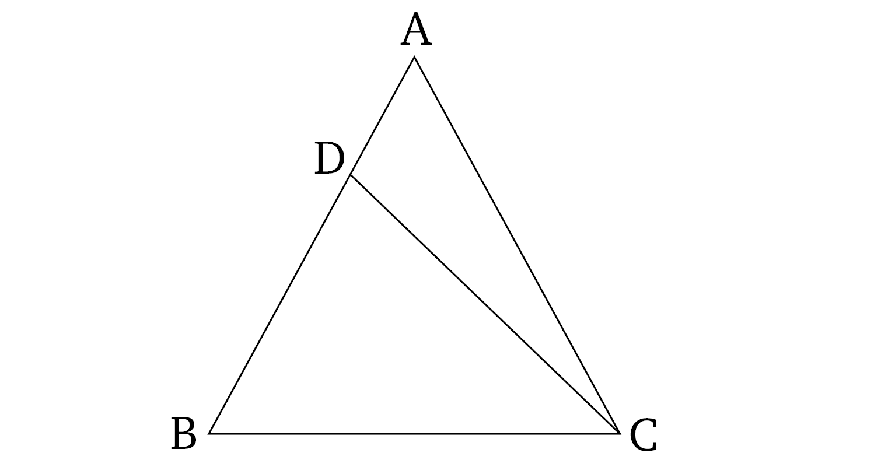
\includegraphics[width=0.55\textwidth]{blaszczyk/bla-fig1a} 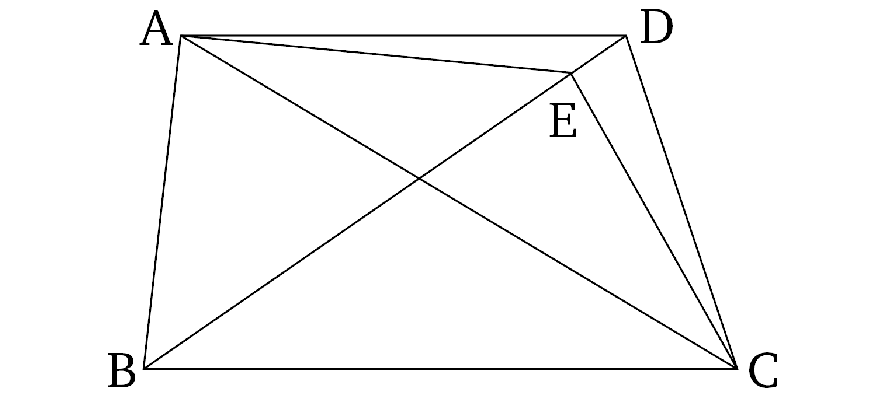
\includegraphics[width=0.55\textwidth]{blaszczyk/bla-fig1b}}
\caption{\textit{Elements}, I.6 (on the left) and 39 (on the right).}
\label{figCN5}
\end{figure}
\subsection{5.2. Mancosu on numerosities}

Paolo Mancosu \parencite*{ref_pm09} is the first study introducing numerosities into a philosophical debate. 
\parencite{ref_pm16} applies numerosities in discussion on the so-called Hume Principle. In what follows, we focus on the former study.


Let start with mathematics. Seeking to present an alternative to Cantor's theory of cardinal numbers, Mancosu adopts labeled sets version, takes $\ell$ to be the identity map, and applies numerosities to subsets of $\N$.\footnote{He refers to \parencites{ref_BN03}{ref_BN06}{ref_BN07} and some other papers. For obvious reasons, he could not refer  to \parencite{ref_BN19}.}

He obtains the extension of natural numbers to hypernatural numbers \mbox{$(\N^*,+\cdot,0,1,<)$} through the ultrapower construction. However, to this end,  following Benci, he applies a selective ultafilter.\footnote{The existence of selective ultrafilters follows from the Continuum Hypotheses. There are models of ZFC with no such filters \parencite[see][76]{ref_tj}} 
Despite involving such strong means, results are a bit below the ones presented in section \S\,4.1 above. 


Mancosu determines numerosity of $\N$ in the same way as we did in section \S\,4.1. So, let us adopt the same notation, $numerosity(\N)=\alpha$. Results regarding odd and even numbers are similar to those presented in section \S\,4.1 above. 
 
 Numerosities of sets $\{kn:n\in\N\}$ and $\{n^2:n\in\N\}$ equal  to  $\alpha/k$, $\sqrt{\alpha}$ respectively. Yet,  it is up to a reader to check why these hyperreal numbers belong to $\N^*$.  In the historical part of the paper, Mancosu discusses Galileo's paradox, yet in the mathematical part, he does not justify the inequality $\sqrt{\alpha}<\alpha$.
 Finally, the paper does not show the numerosity version of Euclid's axiom CN5: $numeosity (A)<numerosity(B)$, given $A\subsetneq B$, although it refers to the part-whole axiom
 in the abstract. 
 
 Determining numerosities, Mancosu  applies the \textit{natural order} of natural 
 numbers.\footnote{See $A_n=\{a : l_A(a)\leq n\}$ \parencite[632]{ref_pm09}.}
 Therefore, Cantor's ordinal rather than cardinal numbers provide  more accurate counterpart for numerosities. 
When discussing G\"{o}del \parencite*{ref_kg47}, he observes: ``G\"{o}del's reflection aims at showing that in generalizing the notion of number from the finite to infinite one inevitably ends up with the Cantorian notion of cardinal number'' \parencite[638]{ref_pm09}. Indeed, that was G\"{o}del's observation. In the same paper, he refers to ordinal numbers, yet, do not find them as extending finite numbers.  However, one can extend the structure of finite numbers, $(\N,+,\cdot, 0,1,<)$,  to cardinal or ordinal numbers. Regarding ordinal numbers, the alternative has been discovered already at the beginning of the 20\textsuperscript{th} century by Gerhard Hessenberg \parencite*{ref_gh06} and his definition of normal sums and products.\footnote{In \parencite[\S\,8]{ref_bf},  we show embedding of ordinal numbers with normal sums and products into the field ONAG.} And indeed, founders of the numerosity project refer to the structure of ordinal numbers with normal sums and products in numerous papers.
 

\subsection{5.3. Mancosu on infinite numbers in a historical context}

The substantial part of \parencite{ref_pm09} consists of a historical survey on mathematical infinity. It is a must-read study for anyone interested in the history of mathematics.  Here, we mention only two issues, which Mancosu omits (maybe intentionally). The first is the tradition of geometrical optics from Euclid to Descartes. In short, it was a dogma of the 17\textsuperscript{th}-century optics that light propagates with infinite velocity. Still, it differed depending on the medium of propagation. 
Consequently, there
was a scale of infinite velocities. Although Descartes faultily believed that light propagates
faster in water or glass than in air, he could establish the ratio of these two
infinities to derive the law of refraction \parencite[see][]{ref_pb20}.

The second issue concerns Cantor's arguments against infinitesimals. Mancosu touches that point regarding Cantor-Bolzano debate. Yet it was Cantor's proxy dispute with Euler and his idea that infinite numbers are inverses of infinitesimals. 
All through his mathematical career, Cantor sought to prove the inconsistency of infinitesimals. Euler in his \textit{Introductio in Analysin Infinitorum} \parencite*{ref_LE48}---the most important treaty in the history of
mathematics---applies both infinitesimals and infinite numbers. Strangely enough, there are only a few references to \parencite{ref_LE48}, of minor importance, in Cantor's papers and letters. 
That bare fact is more significant than Cantor's explicit comments on alternative theories of infinite numbers \parencite[see][]{ref_bf}.

\paragraph{Acknowledgments}
The author is supported by the Polish National Science Centre grant 2018/31/B/HS1/03896.


\end{artengenv}
